% !TEX root = ../thesis.tex
\chapter{Hardware Design}\label{cha:hardware}
After the \gls{FPGA} behavioral simulation is successful, the hardware design process is started.
The initial step is designing a schematic (\cref{sec:sch}) which is followed by the netlist simulation and the placing and routing of components and wires \cref{sec:pr}.
\begin{table}[h]
  \centering
  \renewcommand{\arraystretch}{1.25}
  \caption{All logic \glspl{IC} used in the \gls{EDiC}.}
  \label{tab:cpuIcs}
  \begin{tabularx}{\textwidth}{ |l|r||X| }
    \hline
    \gls{IC}   & Quantity & Function                                                             \\\hline\hline
    74F245     & 17       & Three-State Octal Bus Transceiver                                    \\\hline
    74ABT540   & 14       & Inverting Octal Buffer (\gls{LED} Driver)                            \\\hline
    74F157     & 12       & Quad 2 to 1 multiplexer                                              \\\hline
    74F825     & 10       & Octal register with Three-State, Asynchronous Clear and Clock Enable \\\hline
    74F86      & 7        & Quad XOR                                                             \\\hline
    74F08      & 7        & Quad AND                                                             \\\hline
    74F521     & 6        & 8 bit Inverting Comparator with Enable                               \\\hline
    28C256     & 6        & \gls{EEPROM} with 15 address bits                                    \\\hline
    74ACT245   & 5        & Octal Bus Transceiver used for \gls{SRAM}                            \\\hline
    74F153     & 4        & Dual 4 to 1 multiplexer                                              \\\hline
    74F32      & 4        & Quad OR                                                              \\\hline
    BERG40     & 3        & 40 pin Connector for Test-Adapter                                    \\\hline
    BERG26     & 3        & 26 pin Connector for Test-Adapter                                    \\\hline
    74F151     & 3        & 8 to 1 multiplexer                                                   \\\hline
    74AS867    & 3        & Synchronous 8 bit cascaded counter with loading                      \\\hline
    BERG10     & 2        & 10 pin Connector for Test-Adapter                                    \\\hline
    74F273     & 2        & Octal register with clear                                            \\\hline
    74F04      & 2        & Hex Inverter                                                         \\\hline
    AS6C4008   & 2        & \gls{SRAM} with 19 address bits                                      \\\hline
    5082\_7340 & 2        & hexadecimal display                                                  \\\hline
    74ACT14    & 1        & Hex Inverter with Schmitt Trigger                                    \\\hline
    DS1813-10  & 1        & Reset Generator                                                      \\\hline
    74F374     & 1        & Octal register with output enable                                    \\\hline
    74ABT245   & 1        & Bus driver used for clock and reset                                  \\\hline\hline
    Sum        & 118      & -                                                                    \\\hline
  \end{tabularx}
\end{table}

\section{Schematic}\label{sec:sch}
The full schematics of the hardware design can be found in \cref{cha:schem} in \cref{fig:schPC,fig:schRAM,fig:schMC,fig:schClk,fig:schIO,fig:schReg,fig:schAlu}.
The schematic is created in such a way that the logical connections are easy to understand.
Each \gls{IC} has its pins arranged for easy understanding and the connections have meaningful names to easier understand the logic.

The 74 series of \glspl{IC} is used for the \gls{EDiC}.
However, a lot of decisions need to be made in choosing the correct \glspl{IC} and
\subsection{Register Comparison}
\begin{figure}[t]
  \centering
  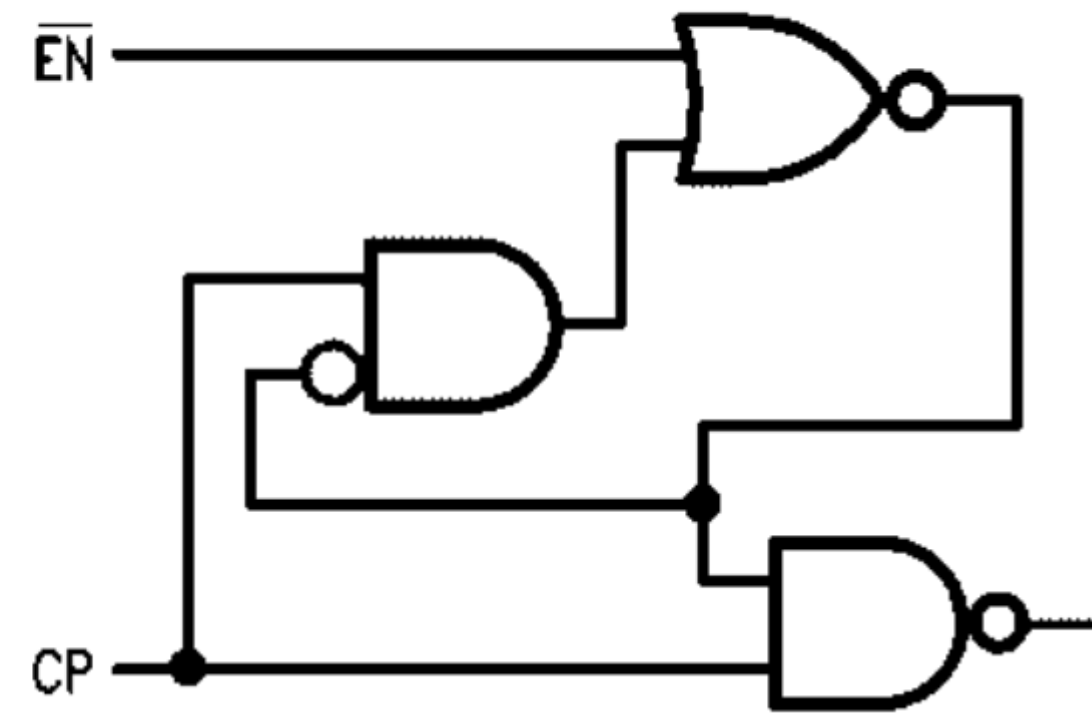
\includegraphics[width=.6\textwidth]{ce.png}
  \caption{Clock Enable circuit of the \emph{74F825} \gls{IC} \cite{74f825}.}
  \label{fig:clockEnable}
\end{figure}
The 74 series of logic \glspl{IC} feature many different registers.
The most basic register \gls{IC} has $n$ D-type flip-flops with respective data inputs and outputs plus one common clock input.
On each rising edge of the clock the flip-flops capture the input values and hold them until the next rising edge of the clock.
However, often it is required that a register does not capture data on every rising edge of the clock.
This is done with an additional input, called \emph{clock enable}.
Implementing the clock enable with a basic AND gate of the clock and a control bit has the major drawback that glitches of the enable control signal can propagate to the clock input of the register and, therefore, falsely trigger the register.
There are two widely used alternatives to the simple AND gate:
The enable input can be used as the select input for an multiplexer to the data input of the flip flop, where it multiplexes between the actual input and the current output.
This allows the flip-flop to always capture data but when the enable input is inactive, it recaptures the current output.
The drawbacks are that each bit of the register needs a multiplexer at the input and, furthermore, that the flip-flops draw power on every clock pulse, even though no new data is captured.
The \emph{74F825} logic \gls{IC} solves this with the circuit shown in \cref{fig:clockEnable}.
When the $\overline{\text{EN}}$ input is low, the CP input is NAND gate on the right passed the negated CP through\footnote{The internal flip-flops of the \emph{74F825} are negative edge triggered}.
When the $\overline{\text{EN}}$ input is high, on the other hand, the output does not change.
This circuit prevents the $\overline{\text{EN}}$ to trigger a falling edge (which would trigger the flip-flops) on the CP output.
However, when the $\overline{\text{EN}}$ goes high while the CP input is high, then the output also goes high.
This is not directly a problem because the flip-flops only trigger on falling edges but is the reason for timing requirements on the $\overline{\text{EN}}$ input which are discussed in more detail in \cref{sec:timing}.
\begin{figure}[t]
  \centering
  \begin{subfigure}[b]{.45\textwidth}
    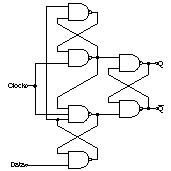
\includegraphics[height=7.5cm]{DFlipFlop.pdf}
    \subcaption{Classical D-type flip-flop built out of three $\overline{\text{SR}}$ NAND latches \cite{DFlipFlop}.}
  \end{subfigure}%
  \hspace{.05\textwidth}
  \begin{subfigure}[b]{.45\textwidth}
    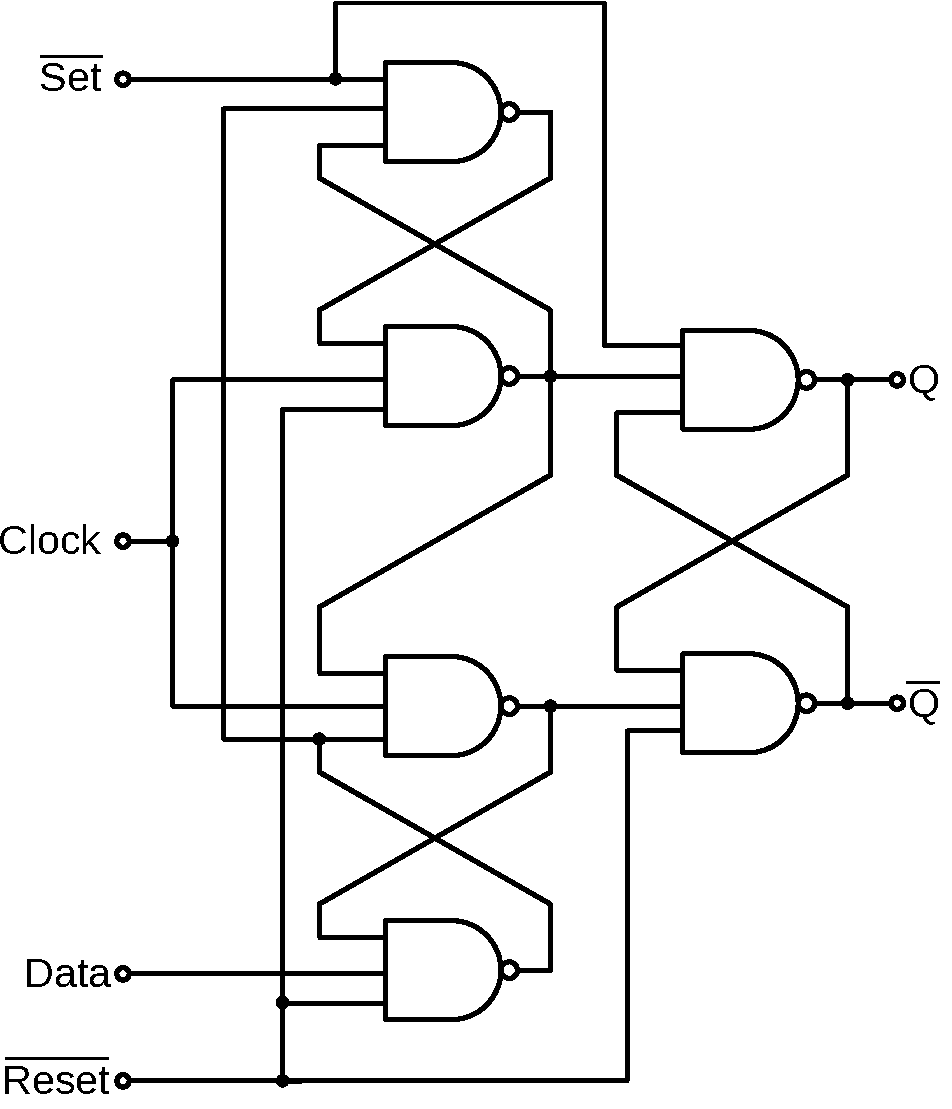
\includegraphics[height=7.5cm]{DFlipFlopClearSet.pdf}
    \subcaption{D-type flip-flop modified to support $\overline{\text{Clear}}$ and $\overline{\text{Set}}$ \cite{DFlipFlopClearSet}.}
  \end{subfigure}
  \caption{Comparison of D-type flip-flops with and without $\overline{\text{Clear}}$ and $\overline{\text{Set}}$.}
  \label{fig:clearSet}
\end{figure}

As the registers store the current state of execution, it is required that the registers start up to a known state.
Therefore, some registers feature an asynchronous clear input (or set input) which forces all flip-flops to 0 (or 1).
This is usually accomplished by modifying the classical D-type flip-flop to allow for setting and resetting the internal $\overline{\text{SR}}$ NAND latches as shown in \cref{fig:clearSet}.

A third feature that may be important is a three-state output which allows the register to be directly connected to a bus.
It is accomplished by adding a tri-state output driver to the outputs of the flip-flops.

The register that was chosen for the \gls{EDiC} is the \emph{74F825} because it has all three features and is 8 bits wide.
However, three other kinds of registers are also sparsely used in the \gls{EDiC}:
\begin{itemize}
  \item The \emph{74AS867} is a more advanced synchronous counter register which is used for the \gls{PC} and \gls{SP}. It is described below.
  \item The \emph{74F374} register only features the output enable and is used once where no additional control logic is required.
  \item The \emph{74F273} is used for the built-in I/O to mimic the typical asynchronous extension cards and for the buffering of user control inputs (stepping etc.).
\end{itemize}

\subsection{LED Driver}\label{sec:ledBuffer}
The \gls{EDiC} features many \glspl{LED} showing the register contents to aid the understanding of the workings of a \gls{CPU}.
However, naively connecting the \glspl{LED} to the logic outputs of registers may lead to unwanted behavior because the outputs of all logic \glspl{IC} have a limited current they can provide.
This leads to the usage of specific buffers for the \glspl{LED}.
Additionally, the current rating usually is higher for low-level output due to the internal workings of the output buffer. % as explained in \cref{sec:outputBuffer}.
For example, the \emph{74F245} non-inverting buffers B output is rated for maximum \qty{-15}{\milli\ampere} for high-level output and \qty{64}{\milli\ampere} for a low-level output \cite{74f245}.
Therefore, connecting the anode of a \gls{LED} via a current limiting resistor to the output of a non-inverting buffer and the cathode to GND will not be ideal.
To be able to draw more current from the buffer and thus having brighter \glspl{LED} inverting buffers are used and the \glspl{LED} are connected ``backwards''.
The \emph{74ABT540} is the \gls{IC} used as \gls{LED} buffer in the \gls{EDiC} with the a low-level current rating of \qty{64}{\milli\ampere} \cite{74abt540}.
The cathodes of the \glspl{LED} are then connected to the \emph{74ABT540} and the anodes are connected through current limiting resistors to $V_{cc}$.

\subsection{Program Counter \& Instruction \glsxtrshortpl{EEPROM}}
\Cref{fig:schPC} contains the \gls{PC} (U54 and U55) with the instruction \glspl{EEPROM} (U62, U67, U69) and the registers to store the instruction.
The \gls{PC} can be incremented or loaded from either an instruction immediate (U50 and U52) for branching or the \gls{SRAM} (U49 and U51) for returning from a function call.
To facilitate these operations, the \emph{74AS867} is used which is an 8 bit synchronous counter with loading and asynchronous clear capabilities that can be cascaded with a ripple carry output.
The \gls{PC} is then used as the address to the instruction \glspl{EEPROM} and can also be saved to the \glspl{SRAM}.
As the main memory is only 8 bits wide but the \gls{PC} 16 bit wide, a second \gls{SRAM} \gls{IC} is used to store the upper bits of the \gls{PC} in the case of a function call (see \cref{sec:schMemory}).
The \gls{PC} is, additionally, used as A inputs to the \emph{74F521} (U53 and U60) comparators to detect when a breakpoint is reached.
The 8 bit comparators can be cascaded via the enable input to compare 16 bit values.
The B input is selected by the user with four hexadecimal digit switches.

The function of the ``Test'' block between the output of the instruction \glspl{EEPROM} and the the instruction registers is explained in \cref{sec:testAdapter}.
For understanding the function of the schematic, it can be assumed that it shorts the connections on the left with the corresponding connections on the right.
The lowest of the 3 instruction registers (U64) holds the instruction code which is used in the \cref{sec:schControl}.
The upper two registers (U70 and U71) hold the immediate value which can be used as an address in the \cref{sec:schMemory}, as a branch address for the \gls{PC} and the lower 8 bits can be used as immediate value on the bus (U75).

All 5 registers have \glspl{LED} connected to them as described in \cref{sec:ledBuffer}.
\subsection{Memory}\label{sec:schMemory}
The memory module (\cref{fig:schRAM}) features three registers used for the address logic:
The \gls{MAR} (U68 and U63) is a 16 bit register where the lower and upper 8 bits can be loaded independently from the bus.
The \gls{SP} (U56) is a \emph{74AS867} counter register as the \gls{PC} but only 8 bits wide and wired differently to only allow incrementing and decrementing.
The three different kinds of memory accesses are decoded from the upper 8 address bits which either come from the instruction immediate (U74) or the \gls{MAR} (U73):
\begin{itemize}
  \item \emph{I/O access:} When the upper 8 bits equal \texttt{0xfe} (U79), the I/O \gls{CE} signal is asserted and the \gls{SRAM} \gls{CE} is deasserted.
  \item \emph{Stack access:} When the upper 8 bits equal \texttt{0xff} (U76), the stack memory is selected.
        Then the upper 8 bits of the address is replaced by the \gls{SP} and a 17th address bit is asserted to access the stack memory.
\end{itemize}
The address is then driven by several bus driver according to the decoding logic (U61, U63, U65, U66 and U72).

The actual \gls{SRAM} \glspl{IC} (U77 and U100) have voltage levels which are not quite compatible with the standard \emph{74F} \glspl{IC} \cite{AS6C4008} which is why all the signals connecting to them are buffered with the \emph{74ACT245} \cite{74act245} (U201, U202, U203, U204 and U205).

\subsection{Control Logic}\label{sec:schControl}
\Cref{fig:schMC} contains two registers for the address of the microcode \glspl{EEPROM} (U85, U86 and U87) of which the data pins are the control signals (\cref{sec:controlSignals}).
The first registers (U83) is used as a synchronous 3 bit step counter which increments each cycle except when the halt signal is asserted.
The instruction finished control signal will reset the step counter to 0 at the next cycle.
U83 also registers the four \gls{ALU} flags and U84 registers the instruction to synchronies all address bits for the \glspl{EEPROM}.

\subsection{Clock and Reset}\label{sec:schClock}
\Cref{fig:schClk} contains the oscillator (X1) which frequency is determined in \cref{sec:timing} and a active low reset controller (U34) which resets on power-on and can be combined with a user reset switch (SW1301).
The clock and reset is buffered with an \emph{74ABT245} for minimal latency.
To avoid glitches (see \cref{sec:switchGlitch}) on the four user inputs, a low pass and a Schmitt trigger and two registers are used.
A multiplexer (U39) generates the halt signal from the debug user inputs and the instruction finished control signal to implement the logic described in \cref{sec:clock}

\subsection{Built-In I/O}
The built-in I/O (\cref{fig:schIO}) consists of one register to hold the output value (U92) which is connected to two hexadecimal displays (U93 and U94).
For input two hexadecimal switches (SW10 and SW11) are used with a bus driver (U91).
To control the register clock pulse and the output enable of the bus driver, the I/O \gls{CE} is combined with the I/O write enable and I/O output enable and the I/O address is compared with \texttt{0x00} (U88).

\subsection{Register Set and \glsxtrshort{ALU} output}
The register set in \cref{fig:schReg} consists of two registers (U40 and U41) which can be loaded from the bus.
The register outputs can drive the bus (U44 and U45) and are multiplexed for the A input of the \gls{ALU} (U42 and U43).
After the combinatorial \gls{ALU} (\cref{sec:schALU}), the four operation results are multiplexed (U5, U6, U7 and U8) and stored in the \gls{ALU} output register (U9).
Even though the \gls{ALU} output register features output enable inputs, an indivual bus driver is used (U10) because the content of the \gls{ALU} output register should be displayed to the user (U11).
The carry flags are also multiplexed (U101) as the carry flag from the shift operation is generated independently.
The overflow flag is generated in the combinatorial schematic of the \gls{ALU}, the negative flag is just the \gls{MSB} of the output and the zero flag is deduced from a comparison with zero (U12).
All four flags are then stored in a register (U97).
\subsection{Combinatorial \glsxtrshort{ALU}}\label{sec:schALU}
\Cref{fig:schAlu} shows the ripple carry adder on the left composed out of 8 full adder and with subtracting capabilities.
The barrel shifter on the right side is explained in depth in \cref{sec:alu}.
The carry flag resulting from a shift operation should always represent the last bit which was shifted out of the 8 bits and should be unchanged when shifting by 0.
This is accomplished with another multiplexer (U102).

\section{Placing and Routing}\label{sec:pr}
\begin{figure}[p]
  \centering
  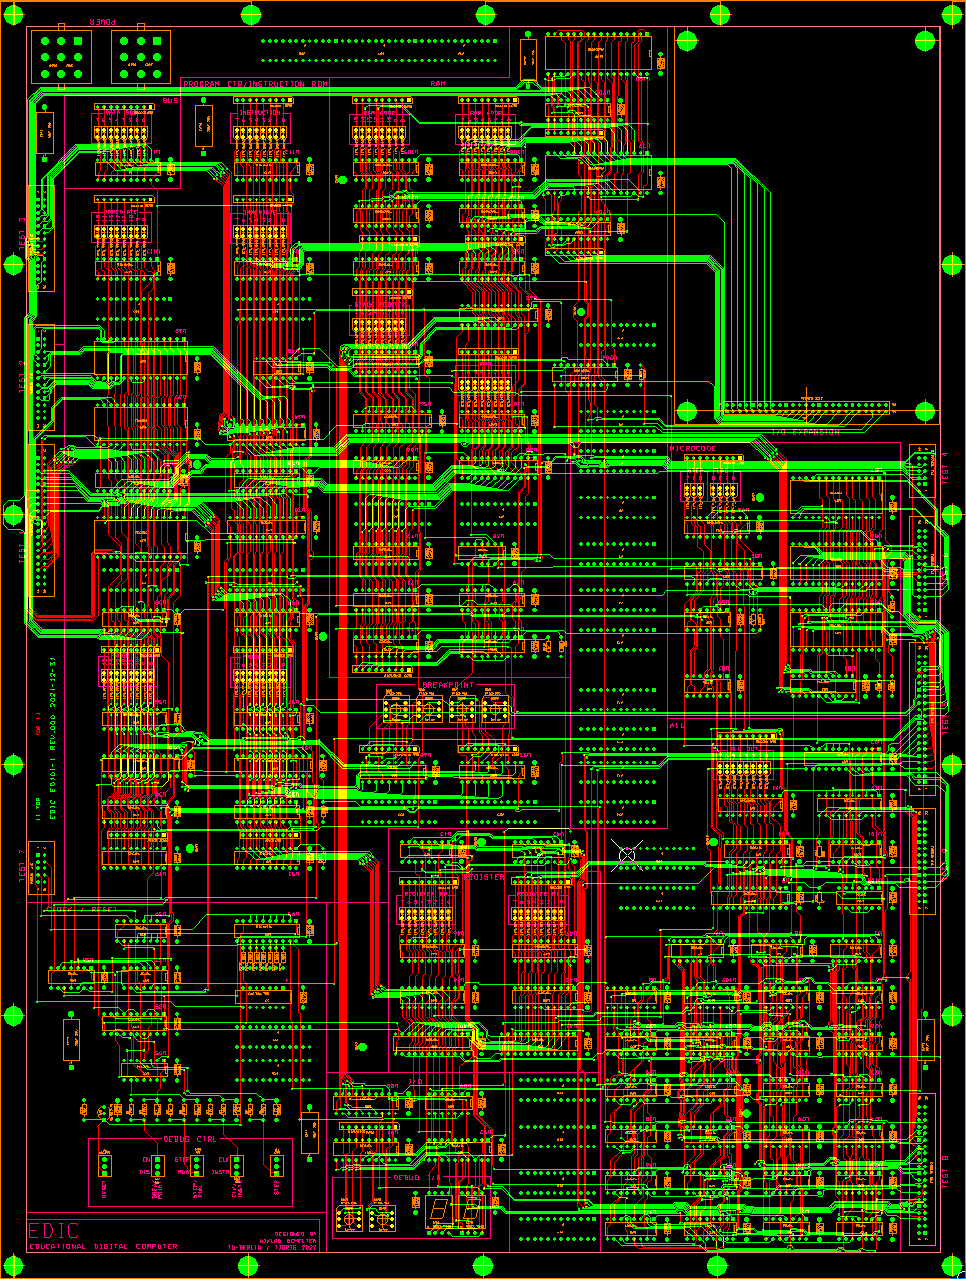
\includegraphics[width=\textwidth]{PR.png}
  \caption{Rendering with all components placed and all the traces routed on the two logic layers (green and red).}
  \label{fig:pr}
\end{figure}
For placing and routing several factors are important.
As the goal of the \gls{EDiC} is to be easy to understand for future students, all components were not only placed to optimize the wiring but also to place components of the same modules close together.
Additionally, extra space was left to mark each module and to name all the \glspl{LED} on the silkscreen of the \gls{PCB} for easier reference.
\Cref{fig:pr} is a rendering showing the traces (red and green), silkscreen (violet) and through-holes/vias (green/yellow).

Especially on larger \glspl{PCB} and designs with quickly switching power consumption it is important to ensure good power delivery to all components.
In the case of the \gls{EDiC} this is achieved by using a 4-layer \gls{PCB} with the two internals layers being filled with GND and 5V panes.
The top and bottom layer are then used for logical connections where the most efficient wiring can be done when one layer mostly has vertical wires (red traces in \cref{fig:pr}) and the other layer mostly horizontal wires (green traces).
This way interference of vertical and horizontal traces is not possible due to the GND and 5V panes separating the logic panes.

Another important factor to bear in mind is to route the traces in a way that makes it possible to access every trace.
It is always possible that some bug was not detected in the schematic design or netlist simulation.
If a bug has been found it may be required to cut a trace and rewire it (see \cref{cha:eval}).
Therefore, logical wires are always placed on the top or bottom pane and on the top pane traces will never be completely covered by \glspl{IC}.
If, for example, connecting pins 1 and 24 of a 24 pin \gls{IC} (they are directly opposite of each other) they should not be connected directly but a detour should be taken to expose the trace from under the \gls{IC}.

It is also possible that a further \gls{IC} needs to be placed on the \gls{PCB} to fix a bug, like an extra register or bus driver.
Therefore, through holes are provided to allow spare \glspl{IC} to be placed at convenient locations throughout the \gls{PCB}.

\section{Timing Analysis}\label{sec:timing}
\begin{figure}[t]
  \centering
  \includegraphics[width=\textwidth]{timingExample.pdf}
  \caption{Timing relations for a combinatorial datapath between two registers.}
  \label{fig:timingExample}
\end{figure}
To figure out what the maximum frequency is at which the \gls{EDiC} can operate on, a detailed timing analysis was performed.
The timing analysis computes the path with the longest propagation delay which called the critical path.
The delay of the critical path can then be used as a baseline for choosing the correct frequency.

\Cref{fig:timingExample} visualizes how the propagation delays work:
Each \gls{IC} has delays which are specified in the datasheet.
In the example of \cref{fig:timingExample}, a value of register $r_0$ goes through a combinatorial path and is then stored in register $r_1$.
The registers have a propagation delay $t_p$ which specifies the time from a rising edge of the clock to the output (Q).
In theory it is also important to hold the input data of a register for the specified hold delay $t_h$, however, in the \gls{EDiC} this is no problem.
Then the combinatorial path also has propagation delays from inputs to outputs which need to be added up ($t_c$).
At the next register, a setup time $t_s$ has to be met which specifies the amount of time the input data needs to be stable before the rising edge.

\begin{figure}[t]
  \centering
  \includegraphics[width=\textwidth]{all_cycles.pdf}
  \caption{Timing analysis for the control signals.}
  \label{fig:timingControl}
\end{figure}
\twopagepicture{p}{ram.pdf}{Timing analysis for the memory latency.}{fig:timingRam}
\twopagepicture{p}{alu.pdf}{Timing analysis for the \gls{ALU} latency.}{fig:timingAlu}
The \cref{fig:timingControl,fig:timingRam,fig:timingAlu} show three timing analysis for the \gls{EDiC}.
Each block represents one \gls{IC} with the corresponding delay.
The first column shows the unit number of the schematic, the second line the type of \gls{IC} and the third shows the kind of delay with the fourth showing the time.
The kind of delay of a buffer can for example be d$\rightarrow$ q which means input data to output data delay or oe$\rightarrow$ q which is the time from asserting output enable until the data is valid.
The delay time is always the worst case time as specified in the datasheet\footnote{Propagation typically varies with the temperature and age of the \gls{IC} and by taking the worst case time (maximum) it is assured that no timings bugs occur due to e.g. weather changes.}.
A vertical double line represents a point where multiple delay paths must be met until the execution can continue.
In \cref{fig:timingControl} for example, the propagation delay of register U83 (flags and step register) and register U84 (instruction) must both be over until the address for the \glspl{EEPROM} U85, U86 and U87 are valid.
At these points the maximum of the merging delay paths is used as the starting point for the next path.
The maximum delay up to this point is also added at the top.
Additionally, some paths are labeled for clarity.
All the times of the critical path (the path that takes the longest from one starting point to one end point) are marked in red.

\Cref{fig:timingControl} shows the basic latency path for control signals and the common bus driver \glspl{IC}.
The latencies inside the register set and program counter are neglectable and, therefore, only the memory module with the complex address decoding and the \gls{ALU} is further examined.
For the memory module (\cref{fig:timingRam}), there are two critical paths:
The first comes from the \texttt{memInstrToRamAddr} control signal, through the stack selection logic to the memory address and finally to the buffered output data of the \gls{SRAM} on the bus (\qty{281.3}{\nano\second}).
The second has the same origin but represents the writing option of the \gls{SRAM} (\qty{272.2}{\nano\second}).

The \gls{ALU} latency path (\cref{fig:timingAlu}) is more complex which is mainly due to the ripple carry adder.
Consequently, the critical path comes from the bus, through all the carry flags to the final adder result.
After the result multiplexer the longest path is from the zero flag to the alu flag register U97 (\qty{313.9}{\nano\second}).

Theoretically, it is possible for one instruction to read a value from the \gls{SRAM} and using it in the same instruction as an input to the \gls{ALU}.
This would replace the baseline delay of the bus input in \cref{fig:timingAlu} (\qty{169.5}{\nano\second}) with \qty{281.3}{\nano\second} and, therefore, enlarge the total worst case latency to
\begin{equation}
  \qty{281.3}{\nano\second}-\qty{169.5}{\nano\second}+\qty{313.9}{\nano\second}=\qty{425.7}{\nano\second}\label{eq:latency}
\end{equation}
Notwithstanding, because the \gls{EDiC} is a multicycle \gls{CPU} it is easily possible to assign two cycles to all \gls{ALU} operations where the B operand is read from the memory.
With this trick, the overall critical path is the maximum of \qty{313.9}{\nano\second} and half of \cref{eq:latency} which is \qty{313.9}{\nano\second}.
With a safety margin of 30\% it is feasible to choose an oscillator with a frequency of \qty{2.4}{\mega\hertz}:
\begin{equation}
  \qty{2.4}{\mega\hertz}\leq\frac{1}{1.3\cdot\qty{313.9}{\nano\second}} =\qty{2.45}{\mega\hertz}
\end{equation}

